\chapter{Implementation}\label{C:impl}

\section{Vivado Setup}

\begin{figure}[H]
    \begin{center}
        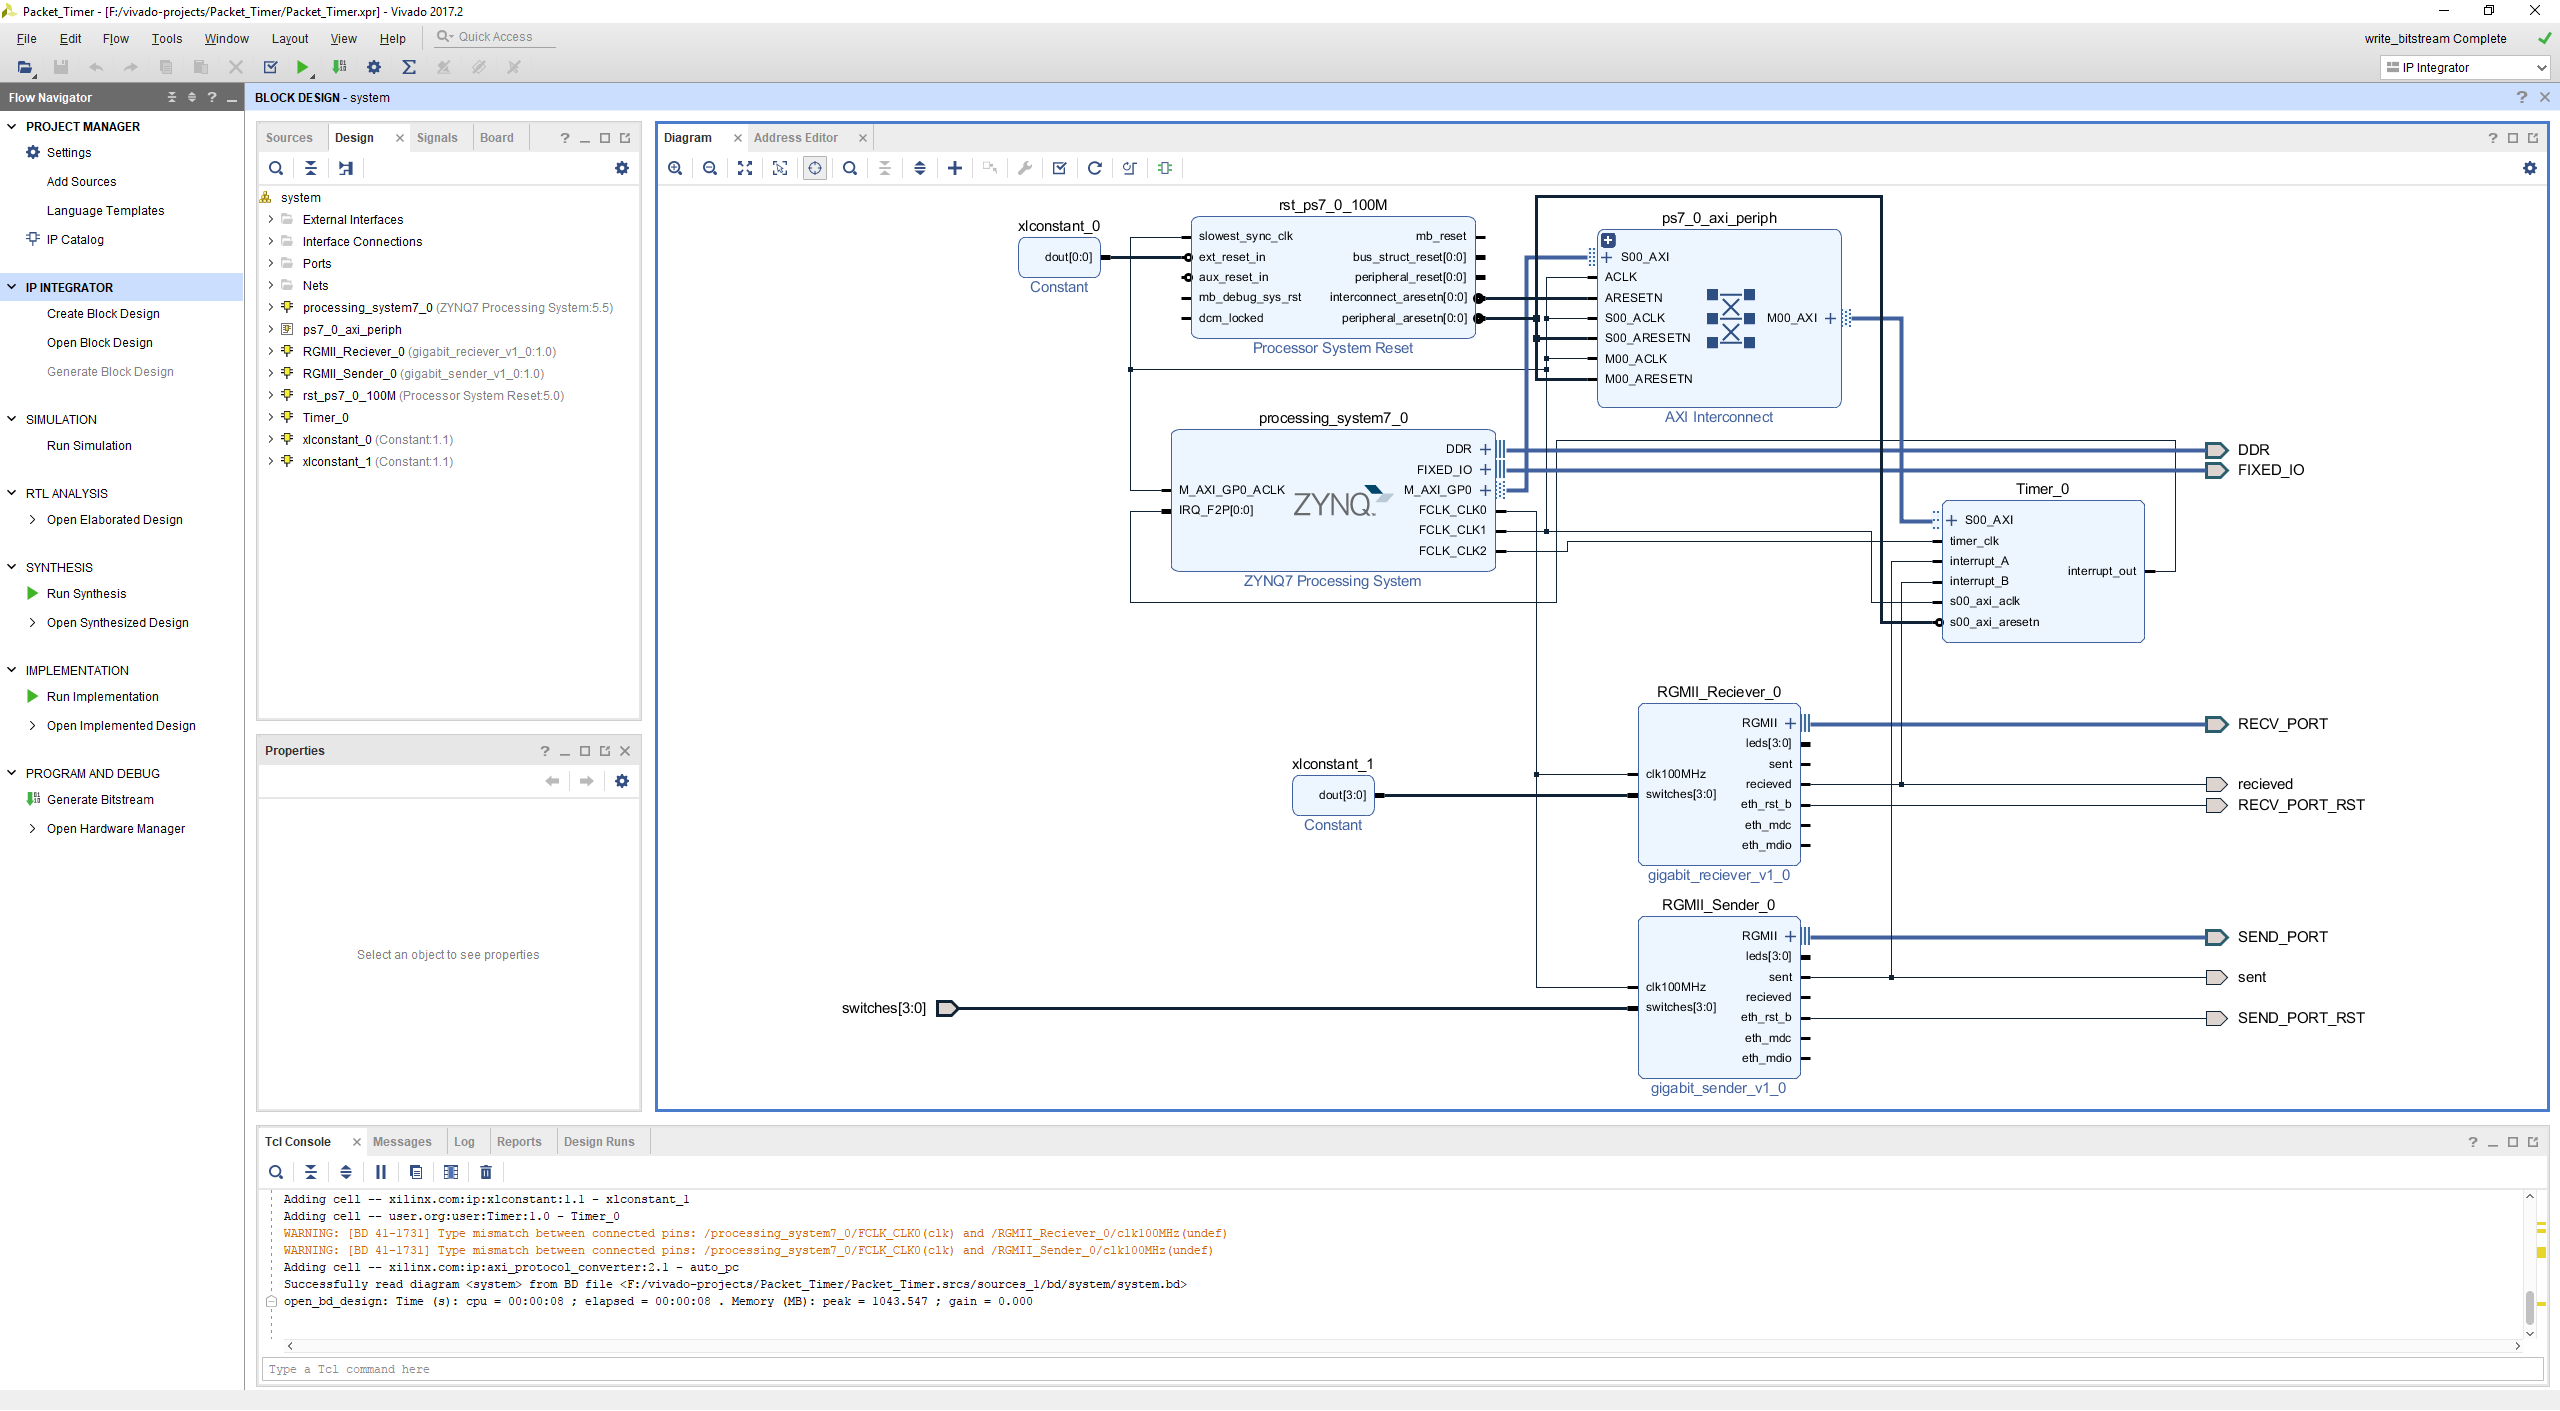
\includegraphics[height=8cm,keepaspectratio]{Images/Vivado.png}
        \caption{Screenshot of Vivado Design Suite 2017.2 User Interface}
        \label{fig:vivado}
    \end{center}
\end{figure}

As the device is using a Xilinx platform, the Xilinx suite of software must be used to create and implement a FPGA 
design for the Zynq FPGA. Vivado Design Suite is the software made by Xilinx which allows for the design and 
evaluation of FPGA designs. To design this project, the Zedboard by AvNET featuring the XC7Z020-CLG484 FPGA was 
chosen as the platform to use as the university had readily available access to resources and help required to 
develop for the board. The WebPACK edition of Vivado allows for the whole software suite to be used, but limited to 
a few devices, under which the XC7Z020-CLG484 is included. Vivado 2017.2 was used for the designing and implementing 
the FPGA design.

\section{VHDL Implementation}

The design of the packet generator was a modified example of a RGMII packet sender was used, which was created by an 
engineer called Mike Field. The original design generated predefined packet structure which mimicked a UDP packet. 

\lstinputlisting[language=VHDL, firstline=16, lastline=41, basicstyle=\small]{Code/gigabit\string_test.vhd}

The leds std\textunderscore logic signal represents a 4 LEDs which show the status of the generator. One LED is used for 
full duplex communication, and the other 3 show the speed of the link (10mb, 100mb and 1000mb). 

\lstinputlisting[language=VHDL, firstline=355, lastline=372, basicstyle=\small]{Code/gigabit\string_test.vhd}

The switches signal control the speed at which the generator creates packets. The switches signal is connected to physical 
on off switches located on the device itself.  This control is an added feature built into the generator code 
beforehand and was kept in the design so the user could select how fast to generate test data.

\lstinputlisting[language=VHDL, firstline=46, lastline=52, basicstyle=\small]{Code/edge\string_detector.vhd}

The modifications made to the generator was to create an interrupt on when the packet is sent and when a packet is 
received. This is done through adding a module which is wired to the RGMII signals themselves and 
produce an output to the sent and received outputs on the top-level module.

\lstinputlisting[language=VHDL, firstline=36, lastline=37, basicstyle=\small]{Code/byte\string_data.vhd}

To ensure that the generated packets are correctly switched through the network switch, the data needs to have the 
correct MAC address for both the destination and sender. The sender address was hard coded into the generator to be 
3C:97:0E:87:D2:42 and the receiver was coded to be 3C:97:0E:87:D2:41.The receiver produces 1 packet per second to assist 
the network switch in adding and entry to the MAC learning table to ensure that the sent packets from the generator 
are not flooded to every port, every time. 

Interrupts for the timing module are created inside the generator and receiver. The sent interrupt is a duplication 
of the signal which activates the chain of data sent to the Ethernet Phy, called start\textunderscore sending. This 
signal goes high when a counter reaches a value corresponding to max\textunderscore count which will activate the 
byte\textunderscore data module and begin sending data to the Ethernet Phy. The Received interrupt is generated when 
the RX\textunderscore CTL line is high when the clock has a rising edge. This is defined in \cite{RGMIISpec} as the point at which the Ethernet Phy has data for the MAC to receive. 

To measure the time between the two interrupts (Sending and receiving) another module is introduced. This module is 
provided with an arbitrary clock which will determine the resolution of the timing. For the purposes of this project,
as 250 MHz clock is used, making the difference between rising edges to be 4ns. When an interrupt is detected on 
the beginning port, a counter begins clocking up for every rising edge of the clock provided. This increments for 
every edge until the second interrupt is asserted high, which stops the counter and this value is stored into a 
register. This register is held with the value until the begin interrupt is asserted again, for which the counter is 
reset to 0 and the process begins again.

The register with the clock value is accessible via the AMBA interconnect using the AXI protocol. This allows the PS 
to access registers (such as the timer value) found in the PL. The PS can request access to the register and 
manipulate the value with software based methods from then on. As the clock frequency in this project is kept at 250 
MHz, the stored register can be interpreted as an unsigned integer that if multiplied by 4, would provide the latency 
in nanoseconds. 

Utilizing software running on the PS, the constant processing time is removed and the xilffs library to communicate 
to the SD card. Using the xilffs library functions, the data is written to the SD card in a simple CSV format, for 
post processing.

\section{Xilinx SDK}

\begin{figure}[H]
    \begin{center}
        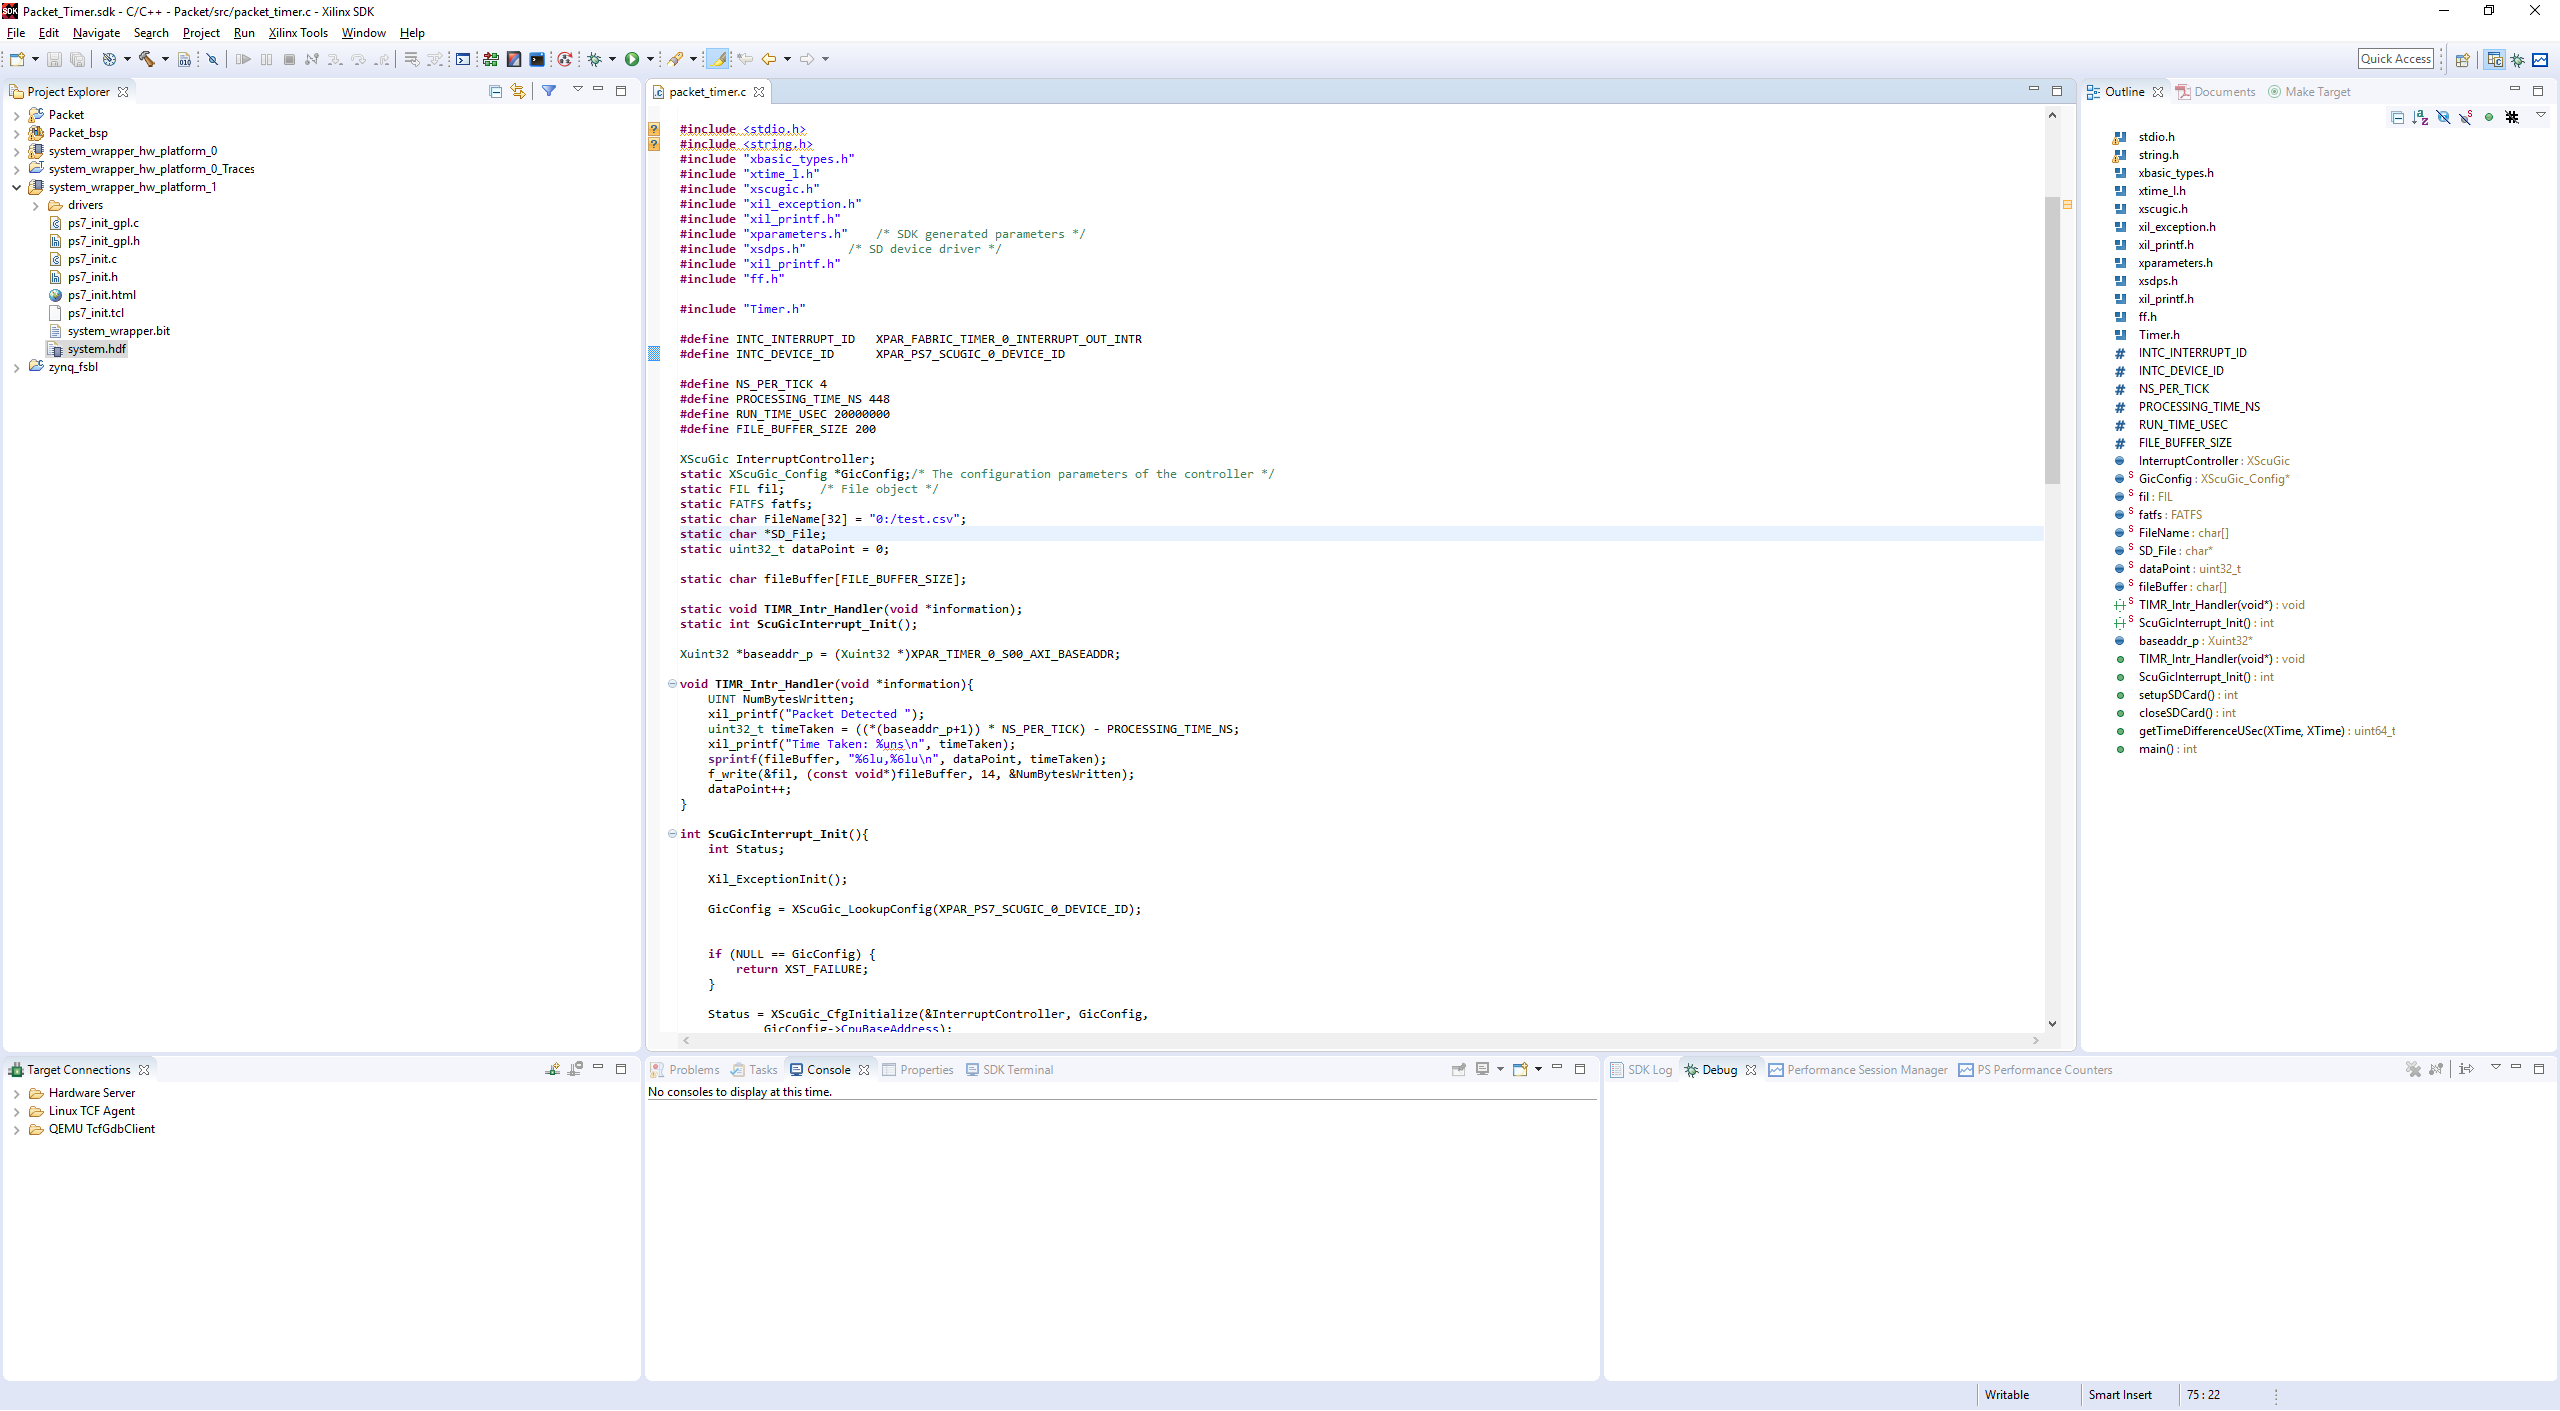
\includegraphics[height=8cm,keepaspectratio]{Images/SDK.png}
        \caption{Screenshot of Xilinx SDK user interface}
        \label{fig:SDK}
    \end{center}
\end{figure}

To run software on the PS of the FPGA, C code is written in the Xilinx SDK and the standard input and output is 
piped through the UART on the FPGA. This C code is also able to interact with PS specific GPIO and peripherals, such 
as the SD card and USB port.  Applications made in the Xilinx SDK are called “Bare Metal” applications, as they 
require no operating system to run on the PS.

To perform a test with the device, a C program has been created which when run, the device produces packets on PORT0 
on the Ethernet FMC and detects the packets on PORT1. The time difference between these is then recorded and 
processed before being written to a CSV file on the SD card. 

